%%%%%%%%%%%%%%%%%%%%%%%%%%%%%%%%%%%%%%%%%
% Stylish Article
% LaTeX Template
% Version 2.2 (2020-10-22)
%
% This template has been downloaded from:
% http://www.LaTeXTemplates.com
% https://www.latextemplates.com/template/stylish-article
%
% Original author:
% Mathias Legrand (legrand.mathias@gmail.com) 
% With extensive modifications by:
% Vel (vel@latextemplates.com)
%
% License:
% CC BY-NC-SA 3.0 (http://creativecommons.org/licenses/by-nc-sa/3.0/)
%
%%%%%%%%%%%%%%%%%%%%%%%%%%%%%%%%%%%%%%%%%

%----------------------------------------------------------------------------------------
%	PACKAGES AND OTHER DOCUMENT CONFIGURATIONS
%----------------------------------------------------------------------------------------

\documentclass[fleqn,10pt]{SelfArx} % Document font size and equations flushed left

\usepackage[english]{babel} % Specify a different language here - english by default

\usepackage{lipsum} % Required to insert dummy text. To be removed otherwise

\usepackage{epigraph}

\usepackage{booktabs}
\usepackage{multirow}
\usepackage[table,xcdraw]{xcolor}
\usepackage{adjustbox}
\usepackage{tablefootnote}
\newcolumntype{C}[1]{>{\centering\let\newline\\\arraybackslash\hspace{0pt}}m{#1}}

\usepackage{./msc}

%----------------------------------------------------------------------------------------
%	COLUMNS
%----------------------------------------------------------------------------------------

\setlength{\columnsep}{0.55cm} % Distance between the two columns of text
\setlength{\fboxrule}{0.75pt} % Width of the border around the abstract

%----------------------------------------------------------------------------------------
%	COLORS
%----------------------------------------------------------------------------------------

\definecolor{color1}{RGB}{0,0,90} % Color of the article title and sections
\definecolor{color2}{RGB}{0,20,20} % Color of the boxes behind the abstract and headings
\definecolor{keys1}{rgb}{0.0, 0.29, 0.33}
\definecolor{keys2}{rgb}{0.25, 0.7, 0.55}
\definecolor{keys3}{rgb}{0.1, 0.3, 0.4}
\definecolor{keys4}{rgb}{0.21, 0.46, 0.53}
\definecolor{strings}{rgb}{0.0, 0.47, 0.44}
\definecolor{comments}{rgb}{0.4, 0.4, 0.5}
\definecolor{terminaltext}{rgb}{1,1,1}
\definecolor{terminalbackground}{rgb}{0.2,0.2,0.3}

%----------------------------------------------------------------------------------------
%	BLOCKS
%----------------------------------------------------------------------------------------

\usepackage[framemethod=TikZ]{mdframed}
\newcounter{definition}[section]\setcounter{definition}{0}
\newcommand{\thedef}{\arabic{section}.\arabic{definition}}
\newenvironment{definition}[2][]{%
    \refstepcounter{definition}
 
    % Code for box design goes here.
	\ifstrempty{#1}%
	% if condition (without title)
	{\mdfsetup{%
	    frametitle={%
	        \tikz[baseline=(current bounding box.east),outer sep=0pt]
	        \node[anchor=east,rectangle,fill=color2!10]
	        {\strut Definition~\thedef};}
	    }%
	% else condition (with title)
	}{\mdfsetup{%
	    frametitle={%
	        \tikz[baseline=(current bounding box.east),outer sep=0pt]
	        \node[anchor=east,rectangle,fill=color2!10]
	        {\strut Definition~\thedef:~#1};}%
	    }%
	}%
	% Both conditions
	\mdfsetup{%
	    innertopmargin=10pt,linecolor=color2!10,%
	    linewidth=1pt,topline=true,%
	    frametitleaboveskip=\dimexpr-\ht\strutbox\relax%
	}
 
\begin{mdframed}[]\relax}{%
\end{mdframed}}

%----------------------------------------------------------------------------------------
%	HYPERLINKS
%----------------------------------------------------------------------------------------

\usepackage{hyperref} % Required for hyperlinks

\hypersetup{
	hidelinks,
	colorlinks,
	breaklinks=true,
	urlcolor=color2,
	citecolor=color1,
	linkcolor=color1,
	bookmarksopen=false,
	pdftitle={Title},
	pdfauthor={Author},
}

%----------------------------------------------------------------------------------------
%	ARTICLE INFORMATION
%----------------------------------------------------------------------------------------

\Subject{Computer Network Security seminar} % Journal information
\AcademicYear{A.Y. 2022/2023} % Additional notes (e.g. copyright, DOI, review/research article)

\PaperTitle{Automated Symbolic Verification of the Needham-Schroeder Protocol} % Article title

\Authors{Denis D'Ambrosi\textsuperscript{1}} % Authors
\affiliation{\textsuperscript{1}\textit{Student number 147681}, \lstinline|dambrosi.denis@spes.uniud.it|} % Author affiliation

\Keywords{Network Security --- Automated Verification --- Formal Verification} % Keywords - if you don't want any simply remove all the text between the curly brackets
\newcommand{\keywordname}{Keywords} % Defines the keywords heading name

%----------------------------------------------------------------------------------------
%	ABSTRACT
%----------------------------------------------------------------------------------------

\Abstract{As cryptographic protocols become both more complicated and more critical by the day, we must find a way to systematically verify message exchanges without the added burden of manual proving. To solve this issue, multiple theorem provers have been proposed in the last years, each one with its flaws and advantages. In this paper, we deal with the Tamarin prover, an automated tool that exploits multiset rewriting rules and guarded fragments of temporal logic to model cryptographic protocols and check their security properties. After an initial introduction to the topic as a whole, we dig deeper into the tool from a user's perspective and show how a simple key exchange protocol (the symmetric Needham-Schroeder protocol) can be modeled within a logic theory. This example will allows us to show how easily some message exchanges can be formalized within this prover; on the other hand, it will also demonstrate how the unbounded nature of this tools will require us to take some further assumptions on the protocol in order to avoid non-termination.}

%----------------------------------------------------------------------------------------
\renewcommand*{\ttdefault}{qcr}
\begin{document}

\maketitle % Output the title and abstract box

\tableofcontents % Output the contents section

\thispagestyle{empty} % Removes page numbering from the first page

%----------------------------------------------------------------------------------------
%	ARTICLE CONTENTS
%----------------------------------------------------------------------------------------

\section*{Introduction} % The \section*{} command stops section numbering

\addcontentsline{toc}{section}{Introduction} % Adds this section to the table of contents

\epigraph{Security protocols are three-line programs that people still manage to get wrong}{Roger M. Needham}

As computing becomes more obiquitous and distributed, we need an ever-increasing amount of cryptographic protocols to allow different parties to share information in a confidential, authenticated and integral way. New communication protocols are being deployed by the day, but most of them have at least some hidden flaw that, once found, can compromise the security of the communication, with potentially catastrophic effects. To avoid such a disaster, our best defense is to actually verify said protocols in some formal model, that will ensure us that, at least within the assumptions of the model itself, the exchange can not be exploited maliciously. Writing these proof by hand is often a cumbersome, long and error-prone process, thus in the last years computer scientists and mathematicians have instead started relying on automated tools that can carry on the demonstration for them. In this essay, we will take a closer look at one of such tools (the Tamarin prover \cite{tamarin}), by presenting its syntax, strengths, limitations and a practical example of modelization.

The essay is structured as follows: in section \ref{sec:SymbolicModel} we will briefly introduce one of such formal verification models, in section \ref{sec:TamarinOverview} we will give an introduction to the Tamarin prover from a user's perspective, while in the following section we will show how such tool can be used for real-world formal verification by modeling the Needham-Schroeder Symmetric protocol. Finally, in section \ref{sec:conclusions} we will summarize the results of this paper.

\section{The symbolic model}\label{sec:SymbolicModel}

Known also as the \textit{Dolev Yao} model, the symbolic model abstracts from cryptography by substituting real-world cryptographic operations with term-algebras \cite{DolevYao}. Encryption schemes are formalized through binary isomorphisms within $\{0,1\}*$: given a symmetrical key $k$ and the relevant pair of cryptographic encryption and decryption primitives $\textrm{senc}_k$ and $\textrm{sdec}_k$, symmetrical cryptography is defined through the following identity:

\begin{equation}\label{eq:SymmetricEncryptionIdentity}
    \textrm{sdec}_k\ \textrm{senc}_k = 1
\end{equation}

Only the entities that are in possess of $k$ are able to encrypt or decrypt any message with it \cite{BBSecurityProtocolVerification}: this assumption is known as perfect cryptography. Furthermore, given a message $M$ and its image $\textrm{senc}_k\ M$, we assume that it is impossible for an attacker who does not know $k$ to:

\begin{itemize}
    \item guess or bruteforce $k$;
    \item manipulate $\textrm{senc}_k\ M$
    \item infer any information about $M$ from $\textrm{senc}_k\ M$.
\end{itemize}

Similarly to equation \ref{eq:SymmetricEncryptionIdentity}, asymmetric encryption and signing are modeled through the following identity:

\begin{equation}\label{eq:AsymmetricEncryptionIdentity}
    \textrm{adec}_{pr}\ \textrm{aenc}_{pub} = \textrm{adec}_{pub}\ \textrm{aenc}_{pr} = 1
\end{equation}

In this case, we do not consider a single key used for both encryption and decryption $k$, but instead an entangled pair of keys $pr$ and $pub$. The assumptions for cryptography are the same as above.

A protocol is modeled as a series of formal terms (messages) exchanged by abstract machines (clients) through an attacker-controlled network. We assume that any connection can be eavesdropped by a malevolent agent that is also able to intercept, modify, forge and drop messages on the fly, with the only exception of the encryption constraints previously described. After formalizing a protocol, its security goals can be expressed as \cite{SoK}:

\begin{itemize}
    \item Trace properties: invariants that should hold for each possible execution of the protocol;
    \item Observational equivalence properties: properties that an attacker should not be able to distinguish between two different runs of the protocol.
\end{itemize}

The use of algebraic terms within the Dolev Yao model allows for simple abstractions during formal checking. As opposed to the aforementioned standard model, where bitstrings take the place of terms and perfect cryptography is not an assumption, the symbolic model is less realistic since it is able to guarantee only high-level security goals on the conjecture of flawless implementations of the cryptographic primitives actually used.

\subsection{Limits of the symbolic model}

In order to streamline the proof of security properties belonging to a certain protocol, multiple automatic tools were proposed \cite{SoK}. These softwares, in order to prove security goals, have to compute the set of terms that an attacker is able to deduce while the protocol is executing, although since this set can possibly be infinite, the general problem suffers of both undecidability and infinite state space. To convince ourselves that this is the case, we just need to think about the fact that we can have an infinite number of sessions for each protocol, each one with different nonces and messages of unlimited size. Without bounding at least two of these sources of infinity, termination can not be guaranteed by any tool in this category.

\begin{figure*}[t]
    \centering
    \captionsetup{justification=centering, margin=1cm}
    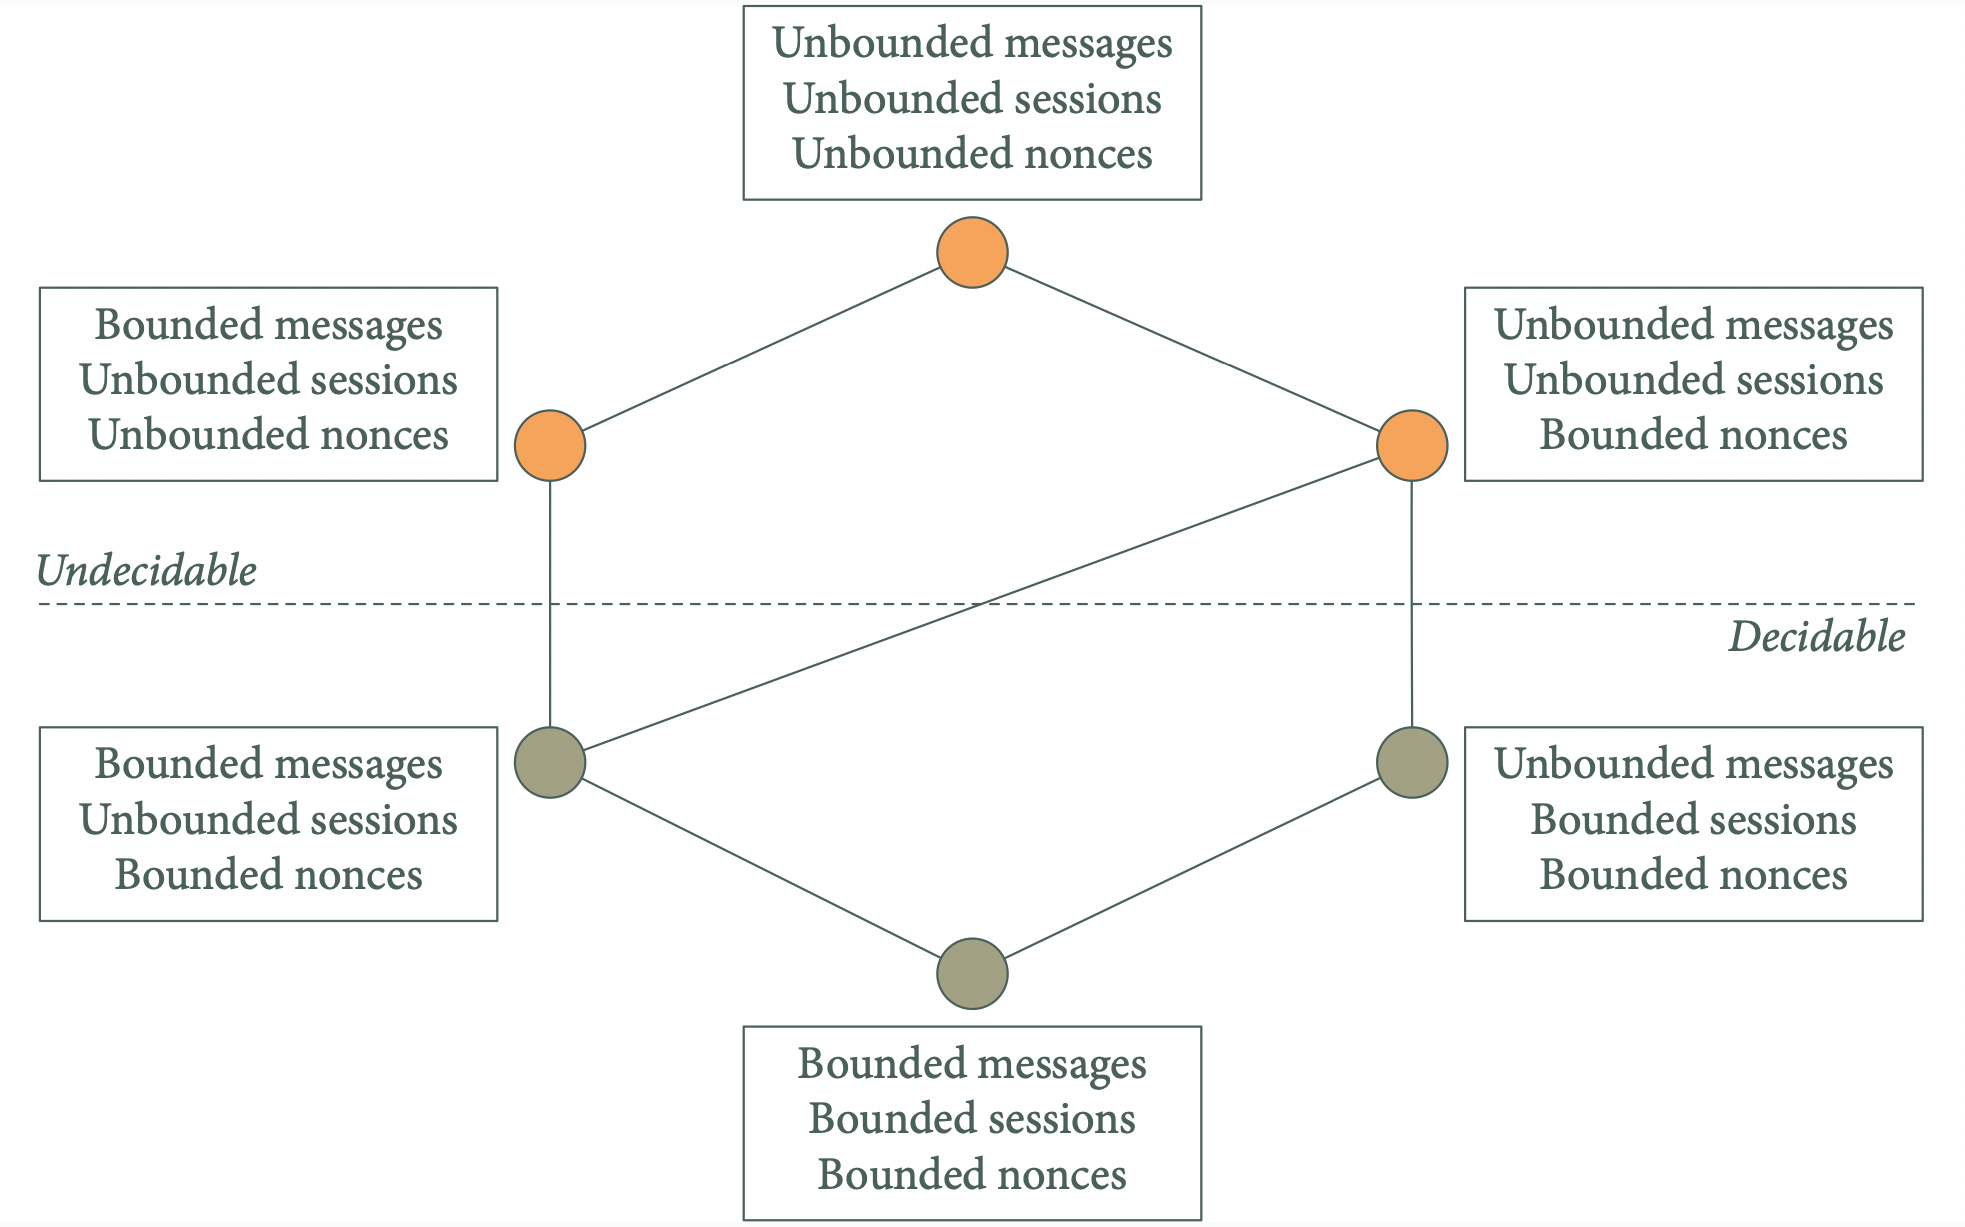
\includegraphics[width=0.8\textwidth]{Figures/undecidability.png}
    \caption{Decidability in symbolic verification. Image taken by N. Vitacolonna's presentation \cite{PresentazioneVitacolonna}}
\end{figure*}


In particular, as shown by N. Durgin et al. \cite{ComplexityOfBoundedSecurity}, by restricting different sources we can ensure to reduce insecurity to different complexity classes:

\begin{itemize}
    \item if we limit the number of nonces and messages, we end up with a DEXP-complete problem;
    \item if we restrict the number of sessions (and thus the number of nonces and messages), the problem will still be affected from infinite state space, but its solution will be NP-complete; this workaround was adopted by a variety of tools such as Cl-AtSe \cite{clAtse}, OFMC \cite{ofmc} and SATMC \cite{satmc}.
\end{itemize}

Alternatively to bounding the sources of infinity, some software address undecidability by requiring human input (for example, Tamarin Prover \cite{tamarinIntroduction} features an interactive mode that allows the user to decide which security goals prioritize based on intermediate constraint systems), returning inconclusive results (for example, ProverIf \cite{proverifIntroduction} may return an invalid attack trace) or even allowing non-termination.

\section{Tamarin Prover Overview}\label{sec:TamarinOverview}

The automatic tool we used to complete the experimentation for this thesis is Tamarin Prover (which from now on we will call Tamarin for the sake of semplicity). We will now do a quick overview of its syntax, semantics and internal functioning; please refer to S. Meier's \cite{meierThesis} and B. Schmidt's \cite{schmidtThesis} PhD thesis and their introductory paper \cite{TamarinFoundations} for further information about the theoretical foundations regarding this tool, as long as its official manual \cite{tamarinManual} to resolve any doubts about its use.

\subsection{Basic definitions}

Tamarin allows protocol (and adversary) modeling through multiset rewriting rules.

\begin{definition}[Multiset rewriting rule]

Given a multiset $\Gamma_t = \{ F_0, ..., F_n \}$ and a sequence of multisets $trace_t = \langle a_0, ..., a_{t-1} \rangle$ at a time $t$, we can define a rewrite rule as a triple of multisets $RR = \langle L, A, R \rangle$ (written as $RR= L -[ A ] \rightarrow R$) such that:

\begin{itemize}
    \item we can apply $RR$ to $\Gamma_t$ if there is at least one ground instance (i.e. an instance with no variables) $rr = l -[ a ] \rightarrow r$ of $RR$ so that $l \subseteq^{\#} \Gamma_t$
    \item applying $rr$ to $\Gamma_t$ yields to a new state $\Gamma_{t+1}$ and an increased trace $trace_{t+1}$ obtained as

\begin{align}
    \Gamma_{t+1} &= \Gamma_t \setminus^{\#} l \cup^{\#} r \label{eq:StateEvolution}\\
    trace_{t+1} &= \langle a_0, ..., a_{t-1}, a_t \rangle
\end{align}

\end{itemize}

in which $\setminus^{\#}$ and $\cup^{\#}$ are the multiset equivalent operations for set difference and union. From now on, we will refer to $L$, $R$ and $A$ as the multisets of \textit{premises}, \textit{conclusions} and \textit{action facts} of a rule (in this order). 
\end{definition}

Note that within the trace $trace_{t+1}$, $a$ is associated to the time istant $t$: this will be useful later on since security properties will be specified through first order logic guarded formulas. To be precise, a \textit{trace} is the sequence of sets of ground (action) facts that happened during the execution of a series of rewriting rules.

More formally, given a set of rules $P$, all the possible traces generated by executions of P are

\begin{align*}
    traces(P) = \{ &\langle A_1,...,A_n \rangle | \exists S_1,...,S_n . \varnothing ^{\#} \xrightarrow[]{A_1} S_1 \xrightarrow[]{A_2} ... \xrightarrow[]{A_n} S_n\\
    & \textrm{and no ground istance of Fresh() is used twice }\}
\end{align*}

For the purpose of this thesis is also worth mentioning that since in a rewriting rule $L -[ A ] \rightarrow R$ any of the three multisets could be empty, a trace in which all istances of $\varnothing^{\#}$ are removed is called an \textit{observable trace}. 

Within Tamarin, all multisets are composed by facts. Facts feature a precise arity, are named with a starting capital letter and can be either \textit{linear} or \textit{persistent}:

\begin{itemize}
    \item linear facts can be consumed only once and are useful to model state transitions and ephemeral messages;
    \item persistent facts can be consumed unlimited times and are optimal to model enduring knowledge (and are prefixed by an exclamation mark). Note that the introduction of persistent facts requires a slight change to equation \ref{eq:StateEvolution}: whereas before all elements of $l$ were removed from $\Gamma_t$, now only the linear facts beloging to $l$ will be subtracted, while persistent facts will never be consumed.
\end{itemize}

In turn, facts are made up of terms, which can be public (prefixed by a \$), freshly created (prefixed by a \textasciitilde{}) or normal messages (note that public and fresh terms are sub-categories of normal messages).

\subsection{Term algebra}

In order to continue explaining Tamarin's functioning, we have to take a look at the theoretical foundations behind the algebraic terms introduced in \ref{sec:SymbolicModel}.

\begin{definition}[Signature]
    A A signature $\Sigma$ is a finite set of functions of defined arity.
\end{definition}

\begin{definition}[$\Sigma$-terms]
    Given a signature $\Sigma$ and a set of variables $\chi$, with $\Sigma \cap \chi = \varnothing$ we can define the set of $\Sigma$-terms $\mathcal{T}_{\Sigma}(\chi)$ as the minimal set such as

    \begin{itemize}
        \item $\chi \subseteq \mathcal{T}_{\Sigma}(\chi)$
        \item $t_1,...,t_n \in \mathcal{T}_{\Sigma}(\chi) \land f/n \in \Sigma \implies f(t_1,...,t_n) \in \mathcal{T}_{\Sigma}(\chi)$
    \end{itemize}

    Note that $f/n$ indicates a function $f$ of arity $n$.

\end{definition}

\begin{definition}[Substitution]
    Given a signature $\Sigma$ and a set of variables $\chi$, with $\Sigma \cap \chi = \varnothing$, a substitution is a function $\sigma: \chi \rightarrow \mathcal{T}_{\Sigma}(\chi)$.
    
    Similarly, given a function $f/n \in \Sigma$, a substitution can be extended to a mapping $\sigma':\mathcal{T}_{\Sigma}(\chi) \rightarrow \mathcal{T}_{\Sigma}(\chi)$ such that

    \begin{equation*}
        f(t_1,...,t_n)\sigma' = f(t_1\sigma,...,t_n\sigma)
    \end{equation*}

\end{definition}

\begin{definition}[Equation over $\Sigma$]
    Given a signature $\Sigma$, a set of variables $\chi$, with $\Sigma \cap \chi = \varnothing$, an equation over $\Sigma$ is a pair of terms $(t,u)$ with $t,u \in \mathcal{T}_{\Sigma}(\chi)$. Note that in this case, the equation would be written $t \simeq u$. In order to break loops while simplyfing terms, equations can be oriented (as $t \rightarrow u$).
\end{definition}

By introducing a set of equations $E$ we can create a congruence relation $=_E$ on terms $t$ and, consequently, equivalence classes $[t]_E$. The congruence relationship is known as an \textit{equational theory}. Introducing equational theories allows us to unify terms based on the quotient algebra $\mathcal{T}_{\Sigma}(\chi) /_{=_E}$: two terms $t,u \in \chi \cup \mathcal{T}_{\Sigma}(\chi)$ are equal in modulo $E$ if and only if they belong to the same class:

\begin{equation*}
    t =_E u \iff [t]_E = [u]_E
\end{equation*}

\begin{definition}[$(\Sigma, E)$-Unification]
    Given a signature $\Sigma$, a set of variables $\chi$, with $\Sigma \cap \chi = \varnothing$ and an equational theory $E$, two terms $t,u \in \mathcal{T}_{\Sigma}(\chi)$ are $(\Sigma,E)$-unifiable if there is at least a mapping $\sigma$ such that $t\sigma =_E u\sigma$.
\end{definition}

Normally, unification modulo theories is undecidable \cite{unificationUndecidability}: thus Tamarin recommends users to only define \textit{subterm convergent theories} to ensure termination, even though the software never actually checks this constraint.

\begin{definition}[Convergent Theory]
    Before defining what a convergent theory is, we have to define both \textit{terminating} and \textit{confluent} theories:

    \begin{itemize}
        \item A terminating theory is an equational theory which ensures that each term has a \textit{normal form} that can be reached through an arbitrary (but finite) number of substitutions.
        \item A confluent theory is an equational theory that ensures that if a term $t$ can be rewritten as both terms $t_1$ and $t_2$, then there must be a fourth term $t'$ that can be reached through an arbitrary number of substitutions from both $t_1$ and $t_2$.
    \end{itemize}

    A convergent theory is an equational theory that is both terminating and convergent.
\end{definition}

\begin{definition}[Subterm Convergent Theory]
    A subterm convergent theory is an equational theory that is convergent and, for each equation $e: L \rightarrow R, e \in E$, $R$ is either ground and in normal form or a proper subterm of $L$.
\end{definition}

Tamarin uses equational theories to model algebraically the cryptographic primitives, such as symmetrical/asymmetrical encryption/decryption, hashing, signing, pair construction/deconstruction, elevation to power, and more. 10 built-in theories are provided to allow the user to easily formalize most cryptographic protocols:

\begin{enumerate}
    \item \lstinline|hashing|
    \item \lstinline|asymmetric-encryption|
    \item \lstinline|signing|
    \item \lstinline|revealing-signing|
    \item \lstinline|symmetric-encryption|
    \item \lstinline|diffie-hellman|
    \item \lstinline|bilinear-pairing|
    \item \lstinline|xor|
    \item \lstinline|multiset|
    \item \lstinline|reliable-channel|
\end{enumerate}

\subsection{Default facts and rules}\label{subsec:DefaultFacts}

Tamarin provides 4 built-in special facts that allow to model the generation and transmission of messages through the network:

\begin{itemize}
    \item \lstinline|Fr(~msg)| allows to create new messages \lstinline|msg|. Note that each value is freshly generated (let us recall that Tamarin allows an infinite number of nonces), so the same ground value can not appear in two different instances of \lstinline|Fr(~msg)|.
    \item \lstinline|K(msg)| indicates that the attacker deduced \lstinline|msg| from the network.
    \item \lstinline|Out(msg)| allows machines to send messages to the network.
    \item \lstinline|In(msg)| allows machines to query the network for incoming messages.
\end{itemize}

These facts are defined through default multiset rewriting rules according to Dolev Yao's assumptions:

\begin{itemize}
    \item \lstinline|[] --[]-> [ Fr(~msg) ]| allows for the generation of new fresh values.
    \item \lstinline|[ Fr(~msg) ] --[]-> [ K(~msg) ]| allows for the generation of new fresh values by the attacker.
    \item \lstinline|[ Out(msg) ] --[]-> [ K(msg) ]| allows the attacker to eavesdrop all messages travelling through the network. 
    \item \lstinline|[ K(msg) ] --[ K(msg) ]-> [ In(msg) ]| allows user to retrieve messages from the attacker-controlled network.
    \item \lstinline|[] --[]-> [ K($x) ]| allows the attacker to discover all public names.
    \item \lstinline|[ K(x1,...,xn) ] --[]-> [ K(f(x1,...,xn)) ]| allows the attacker to apply $n$-ary functions to arguments he already knows.
\end{itemize}

\subsection{Trace properties}\label{subsec:TraceProperties}

As previously anticipated, in Tamarin security properties are expressed as guarded fragments of first order logic. The syntactical construct adopted by Tamarin to indicate a property to prove is \lstinline|lemma|. Lemmas can be either of type \lstinline|exists-trace|, which are demonstrated by finding a single valid protocol trace verifing the formula, or \lstinline|all-traces|, which are proved by negating the property and trying to find a counterexample. To specify a lemma, we can combinate the following atoms:

\begin{itemize}
    \item false $\bot$;
    \item logical operators $\neg\  \wedge\  \vee\ \implies$;
    \item quantifiers and variables $\forall\ \exists\ a\ b\ c$;
    \item term equality $t_1 \approx t_2$;
    \item time point ordering and equality $i < j$ and $i = j$;
    \item action facts at time points $F @ i$ (for an action fact $F$ at timepoint $i$).
\end{itemize}

Keeping in consideration that also properties can define sets of traces similarly to protocol rules, we can define correctness as follows:

\begin{definition}[Correctness]
    Given a set of protocol rules $P$ and a property to prove $\phi$, $P$ is correct in regards to $\phi$ if and only if the set of traces generated by $P$ is a subset of the one generated by $\phi$:

    \begin{equation*}
        P \vDash \phi \iff traces(\phi) \subseteq traces(P)
    \end{equation*}

    On the contrary, if $P \nvDash \phi$, all traces belonging to $traces(P) / traces(\phi)$ represent valid attacks.
\end{definition}

Note that property proving is done by Tamarin through \textit{constraint systems} resolving. In turn, these systems are simplified by executing a backwards search within the relative protocol's \textit{dependencies graph} (a graph that, for each fact used by a Tamarin \textit{theory}, describes the list of possible rules usable to obtain it). The theoretical foundations behind property proving are beyond the scope of this thesis, but are explained in detail in \cite{schmidtThesis} \cite{meierThesis}. As end users, we can be satisfied by knowing that Tamarin's verification algorithm, although does not guarantee termination, is both \textit{sound} and \textit{complete} \cite{schmidtThesis} \cite{meierThesis} \cite{xorCompleteness}.

\subsection{Observational equivalence properties}\label{subsec:ObsEqProperties}

When operated in \textit{Observational Equivalence Mode} (refer to the official documentation \cite{tamarinManual} for further reference), Tamarin allows for the use of the \lstinline|diff/2| operator \cite{tamarinObsEquivalences}, that permits to demonstrate \textit{diff equivalence} properties. To understand what a diff equivalence property is, we have to firstly introduce the concept of \textit{trace equivalence}

\begin{definition}[Trace equivalence]
    Two different protocols $P_1, P_2$ are trace equivalent if and only if for each trace of $P_1$ exists a trace of $P_2$ so that the messages exchanged during the two executions are indistinguishable.
\end{definition}

This is the weakest (and thus most suitable for security verification) form of observational equivalence. Since many problems in this category are undecidable in nature \cite{traceObservableProperties}, Tamarin only allows diff equivalences in aid of termination.

\begin{definition}[Diff equivalence]
    Two protocols $P_1, P_2$ are diff-equivalent if and only if they have the same structure and differ only by the messages exchanged.

    Thus, the two protocol have the same structure during execution.
\end{definition}

The previously introduced \lstinline|diff(left, right)| operator allows to define a protocol rule that can be instantiated either with the \lstinline|left| or \lstinline|right| value. For each one of them, Tamarin constructs the relative dependencies graph and checks if they are equivalent, which is a sufficient criterion for observational diff-equivalence. Please note that a formal definition of \textit{dependencies graph equivalence}, along with the subsequent demonstration of sufficiency are available in the introductory paper for the observational equivalences in Tamarin written by D. Basin, J. Dreier and R. Sasse \cite{tamarinObsEquivalences}.

\subsection{Aiding termination}

Since protocol verification is an inherently undecidable problem, Tamarin provides some additional functionalities engineered to aid termination.

\subsubsection{Source lemmas}

As explained before, Tamarin elaborates the dependencies graph related to a theory before beginning constraint solving. Since the prover uses an untyped system, in certain cases it is not able to deduce the source of one or more facts, causing partial deconstructions. As explained by V. Cortier \cite{autosources}, for example, this situation occurs whenever the same message has to travel across the network multiple times. To mitigate this issue, Tamarin allows to define a lemma with the additional tag \lstinline|[sources]|, which is automatically proved during the precomputation phase and allows to declare the origin of one or more messages.

An example of this type of lemma, along with its explanation, will be provided in section \ref{subsec:termination}

Note that V. Cortier, S. Dealune and J. Dreier proposed an algorithm for automatic source lemma generation \cite{autosources} that has already been integrated in Tamarin (run the program with the additional \lstinline|--auto-sources| tag to execute the extension), but sometimes it leads to non-termination during the precomputation phase.

\subsubsection{Oracles}

During constraint-solving, Tamarin uses its built-in \textit{smart} heuristic (refer to the relevant section of the manual \cite{tamarinManual} for further reference) to sort the list of security goals to check. Sometimes, though, the algorithm prioritizes the wrong goals, leading to loops in the search and thus to non-termination. In an attempt to prevent this behavior, Tamarin provides also two variants of the \textit{consecutive} heuristic, which guarantee to avoid delaying any goal infinitely to exclude starvation. This causes bigger proofs and still fails to solve the problem sometimes.

By knowing how to manually guide the search (for example after doing some practice with the built-in interactive mode), we can code (in any programming language of choice) an external \textit{oracle}, which will be automatically run by the prover to determine the right priority objective to solve within a list of current goals. This user-defined software receives the name of the lemma and the indexed goal list (sorted by the smart heuristic) as input, and returns the re-ranked list (or, alternatively, only its first element) as output. Note that oracles are generally stateless: for each step of the proof, the program is executed from scratch, with only the name of the considered lemma and the list of current security goals as input.

\subsubsection{Interactive mode}

The Tamarin interactive mode is a powerful feature that enables users to guide the proof search process and interactively inspect the demonstration as it is being constructed. When using the interactive mode, users can provide hints and guidance to the Tamarin prover, which can significantly speed up the proof search process and help to identify any potential issues or vulnerabilities in the security protocol being analyzed. For example, by interleaving automatic steps and manual selection of goals to solve, the user can understand if the tool is entering an infine loop of computation or not by monitoring wheter recursive structures of terms are being produced or not. Furthermore, by guiding the proof, the consumer can easily guess how to build an effective oracle to speed up lenghty proofs. Additionally, the interactive mode provides a valuable opportunity to gain a deeper understanding of how the Tamarin prover works and how it constructs proofs for security protocols. An example of Tamarin in action in interactive mode is displayed in figure \ref{fig:interactive}.

\begin{figure*}
    \centering
    \captionsetup{justification=centering, margin=1cm}
    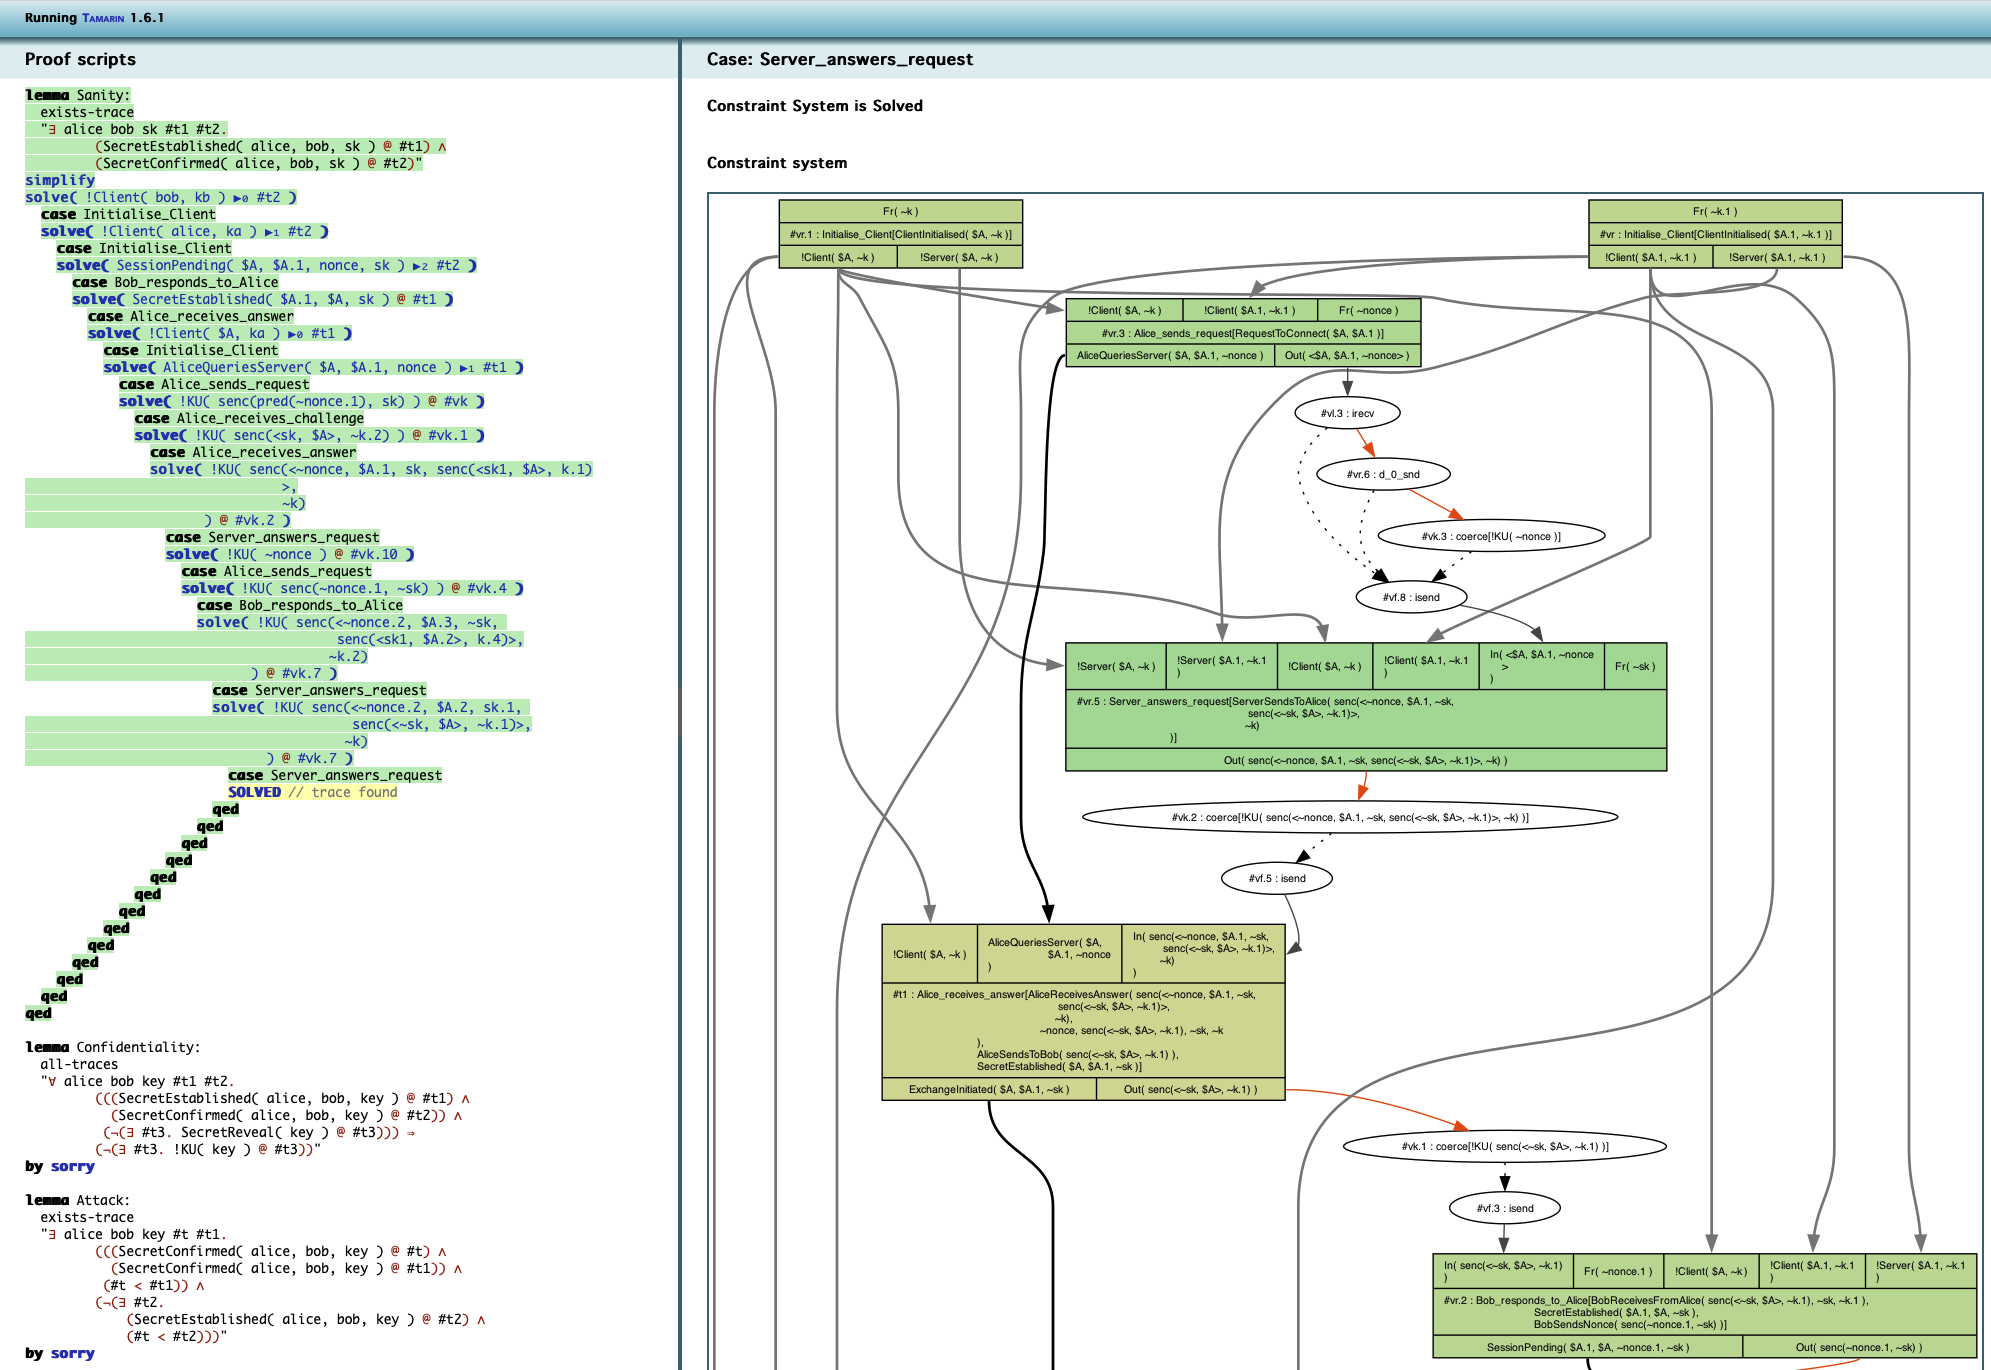
\includegraphics[width=0.8\textwidth]{Figures/gui.png}
    \label{fig:interactive}
    \caption{Tamarin's interactive mode}
\end{figure*}

\subsubsection{Restrictions}

Similarly to lemmas, \textit{restrictions} are specified through guarded fragments of first order logic. The difference between the two is that while lemmas express properties to prove, a restriction limits the possible traces of a protocol to the executions that verify the specified formula.

\subsubsection{Re-use lemmas}

Finally, the last functionality we introduce are \textit{re-use lemmas}: defined with the \lstinline|[reuse]| keyword, these formulas, once proved, can be used by Tamarin in the demonstration of the subsequent specified lemmas.

\section{The Needham-Schroeder Protocol}

The Needham-Schroeder protocol is a key exchange protocol that was introduced in 1978 by Roger Needham and Michael Schroeder \cite{needhamschroeder} to address the issue of authentication in distributed computer networks using symmetric key cryptography.

The Needham-Schroeder protocol is used to establish a shared symmetric key between two parties in a networked environment. The exchange assumes that both parties already have a shared secret with a trusted third party, referred to as a key distribution center (KDC). The KDC is responsible for generating and distributing secret keys to each party, and it also has a public key that can be used to verify the authenticity of messages sent by the KDC.

In the Needham-Schroeder protocol, when one party (Alice) wants to communicate securely with another party (Bob), she sends a request to the KDC for a session key to use in the communication. The KDC then generates a new session key and sends it to Alice encrypted using Bob's public key. Alice can then decrypt the session key using her shared secret with the KDC, and use it to communicate with Bob.

The protocol also includes a mechanism for mutual authentication, which ensures that each party is who they claim to be. When Alice receives the session key from the KDC, she sends a message to Bob that includes the session key and a nonce (a random number). Bob then encrypts the nonce with the session key and sends it back to Alice. Alice can then decrypt the message and verify that the nonce matches the one she sent to Bob. This process ensures that both parties have successfully authenticated each other, and they can begin communicating securely using the session key. The exchange is summarized in diagram \ref{fig:NS}.

\begin{figure}[h]
    \centering
    \captionsetup{justification=centering, margin=1cm}
    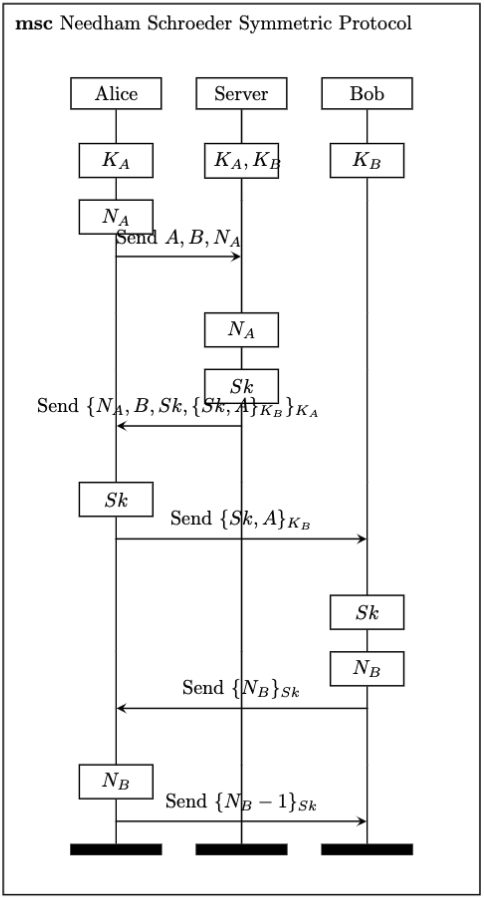
\includegraphics[width=0.45\textwidth]{Figures/NS.png}
    \label{fig:NS}
    \caption{Needham-Schroeder Symmetric protocol}
\end{figure}
%\begin{msc}{Needham Schroeder Symmetric Protocol}
    \declinst{alice}{}{Alice}
    \declinst{server}{}{Server}
    \declinst{bob}{}{Bob}
    \action*{ \begin{minipage}{1cm}\centering $K_A$ \end{minipage} }{alice}
    \action*{ \begin{minipage}{1cm}\centering $K_A, K_B$ \end{minipage} }{server}
    \action*{ \begin{minipage}{1cm}\centering $K_B$ \end{minipage} }{bob}
    \nextlevel[2]
    \action*{ \begin{minipage}{1cm}\centering $N_A$ \end{minipage} }{alice}
    \nextlevel[2]
    \mess{Send $A, B, N_A$}{alice}{server}
    \nextlevel[2]
    \action*{ \begin{minipage}{1cm}\centering $N_A$ \end{minipage} }{server}
    \nextlevel[2]
    \action*{ \begin{minipage}{1cm}\centering $Sk$ \end{minipage} }{server}
    \nextlevel[2]
    \mess{Send $\{N_A, B, Sk, \{Sk, A\}_{K_B} \}_{K_A}$}{server}{alice}
    \nextlevel[2]
    \action*{ \begin{minipage}{1cm}\centering $Sk$ \end{minipage} }{alice}
    \nextlevel[2]
    \mess{Send $\{Sk, A\}_{K_B}$}{alice}{bob}
    \nextlevel[2]
    \action*{ \begin{minipage}{1cm}\centering $Sk$ \end{minipage} }{bob}
    \nextlevel[2]
    \action*{ \begin{minipage}{1cm}\centering $N_B$ \end{minipage} }{bob}
    \nextlevel[2]
    \mess{Send $\{N_B\}_{Sk}$}{bob}{alice}
    \nextlevel[2]
    \action*{ \begin{minipage}{1cm}\centering $N_B$ \end{minipage} }{alice}
    \nextlevel[2]
    \mess{Send $\{N_B-1\}_{Sk}$}{alice}{bob}
\end{msc}

While the Needham-Schroeder protocol is widely used in computer security, it is not without its flaws. One issue is the potential for a "replay attack," where an attacker intercepts and reuses a previously transmitted message to gain access to the network. Another issue is the reliance on a trusted third party, which can be a single point of failure if compromised.

To address these issues, Needham and Schroeder later extended their protocol to include public-key cryptography, resulting in the Needham-Schroeder Public-Key Protocol. This protocol addressed the weaknesses of the original protocol by using public-key cryptography to establish the authenticity of each party's public key and ensure the confidentiality and integrity of the communication.

\subsection{Tamarin Formalization}

\subsubsection{The protocol}

Formalizing the Needham-Schroeder exchange in Tamarin is quite straightforward thanks to the built-in functions and simple syntax provided by the tool (note that all the source files of this section are available for local verification at \cite{github}).

\paragraph{Initialisation}

The clients (Alice and Bob) and the server are initialised with the shared secrets through the following rule:

\begin{lstlisting}[language=Tamarin]
rule Initialise_Client :
    [
        Fr(~k)
    ]
    --[ ClientInitialised($A, ~k) ]->
    [
        !Client($A, ~k),
        !Server($A, ~k$)
    ]
\end{lstlisting}

Note that since we do not have any particular reason to believe that identities are private, we must formalize them as public names known to the attacker. To avoid that the same client gets instantiated twice with two different keys, we exploit the \lstinline|ClientInitialised| action-fact in the following restriction:

\begin{lstlisting}[language=Tamarin]
restriction EachClientCanBeInitialisedOnce :
    "All client key1 key2 #t1 #t2 .
        ClientInitialised(client, key1) @ #t1 &
        ClientInitialised(client, key2) @ #t2
            ==> #t1 = #t2"
\end{lstlisting}

\paragraph{$A \to S: A,B,N_A$}

The first message sent by Alice to initiate the protocol is easily modelled through the following rule (and restriction):

\begin{lstlisting}[language=Tamarin]
rule Alice_sends_request :
    [
        !Client(alice, ka),
        !Client(bob, kb),
        Fr(~nonce)
    ]
    --[ RequestToConnect(alice, bob) ]->
    [
        AliceQueriesServer(alice, bob, ~nonce),
        Out(<alice, bob, ~nonce>)
    ]

restriction NoSelfCommunication:
    "All client #t .
        RequestToConnect(client, client) @ #t ==> F"
\end{lstlisting}

There are multiple elements that we should analyze within this snippet:

\begin{itemize}
    \item The restriction \lstinline|NoSelfCommunication| exploits the \lstinline|RequestToConnect| action fact to restrict connections to only different parties. This is done to prevent Tamarin to waste resources in analyzing self-communicating runs of the protocol, which would be useless in a key-exchange scenario.
    \item This rule also models the generation of the nonce $N_A$.
    \item The fact \lstinline|AliceQueriesServer| will then be useful, once Alice will receive the server's response, to ensure that she was actually the one which initiated the protocol with a fresh nonce before.
\end{itemize}

\paragraph{$S \to A: \{N_A, B, Sk, \{Sk, A\}_{K_B} \}_{K_A}$}

Similarly, the role of the server in the exchange can be modelled through a single rule:

\begin{lstlisting}[language=Tamarin]
rule Server_answers_request :
    let
        message_to_bob = senc(<~sk, alice>, kb)
        message_to_alice = senc(<nonce, bob, ~sk, message_to_bob>, ka)
    in
    [
        !Server(alice, ka),
        !Server(bob, kb),
        !Client(alice, ka),
        !Client(bob, kb),
        In(<alice, bob, nonce>),
        Fr(~sk)
    ]
    --[ ServerSendsToAlice(message_to_alice) ]->
    [
        Out(message_to_alice)
    ]
\end{lstlisting}

Here we exploit the symbolic function primitive \lstinline|senc| included in the built-in \lstinline|symmetric-encryption| equational theory to model the encrypting procedure executed by the server. The action-fact \lstinline|ServerSendsToAlice| will be later used within a source lemma to solve Tamarin's partial deconstruction problem within this theory.

\paragraph{$A \to B: \{Sk, A\}_{K_B}$}

Here we formalize the message sent from Alice to Bob containing the shared secret key generated by the server.

\begin{lstlisting}[language=Tamarin]
rule Alice_receives_answer :
    let
        message_to_bob = senc(<sk1, alice>, k)
        message_to_alice = senc(<nonce, bob, sk, message_to_bob>, ka)
    in
    [
        !Client(alice, ka),
        AliceQueriesServer(alice, bob, nonce),
        In(message_to_alice)
    ]
    --[ AliceReceivesAnswer(message_to_alice, nonce, message_to_bob, sk, ka),
        AliceSendsToBob(message_to_bob),
        SecretEstablished(alice, bob, sk) ]->
    [
        ExchangeInitiated(alice, bob, sk),
        Out(message_to_bob)
    ]
\end{lstlisting}

Similarly to before, the \lstinline|AliceQueriesServer| fact is consumed to produce an analogous \lstinline|ExchangeInitiated| fact, that will be later on used to keep a copy of the shared key and to ensure that Alice actually initiated an exchange if the subsequent messages will come through.

Note that, due to Tamarin's ability to manage an unbounded number of messages, here we had to take a little shortcut in the formalization to force termination during proofs: Alice is not actually able to check the content of the \lstinline|message_to_bob|, since she does not have a copy of his private key $K_B$, but here we use pattern matching to ensure that at least her identity is part of a message structured according the protocol specification. This assumption does not allow us to prove the security properties of the protocol without a little loss of generality, but it is crucial to avoid that Tamarin tries to find an attack trace with an infinite nested sequences of messages. Note that we did not enforce any pattern matching on $K_B$ and $Sk$ to avoid taking any further assumption.

Again, the \lstinline|AliceReceivesAnswer| and |AliceSendsToBob| action-facts will be exploited in the final sources lemma, while \lstinline|SecretEstablished| will be useful to specify the security properties later on.

\paragraph{$B \to A: \{N_B\}_{Sk}$}

Now we can model the challenge of Bob to Alice:

\begin{lstlisting}[language=Tamarin]
rule Bob_responds_to_Alice :
    let
        message_from_alice = senc(<sk, alice>, kb)
        encrypted_nonce = senc(~nonce, sk)
    in
    [
        In(message_from_alice),
        Fr(~nonce),
        !Client(alice, ka),
        !Client(bob, kb),
        !Server(bob, kb)
    ]
    --[ BobReceivesFromAlice(message_from_alice, sk, kb),
        SecretEstablished(bob, alice, sk),
        BobSendsNonce(encrypted_nonce) ]->
    [
        SessionPending(bob, alice, ~nonce, sk),
        Out(encrypted_nonce)
    ]
\end{lstlisting}

Following the structure of the previous rules, we can see that the formalization of this part of the exchange is pretty straightforward. The \lstinline|SessionPending| fact is useful to keep track of the run of the protocol from the point of view of Bob, while the \lstinline|BobReceivesFromAlice| and \lstinline|BobSendsNonce| action fact are necessary to ensure solving partial deconstructions. Finally, this \lstinline|SecretEstablished| fact will be used to specify a "sanity check" of the protocol via an \lstinline|exists-trace| lemma.

\paragraph{$A \to B: \{N_B - 1\}$}

We still need to formalize the last exchange. In order to model the answer to Bob's challenge, we need to define a custom function to have the predecessor function at our disposal within the theory: the following snippet will provide both such definition (that, due to Tamarin's syntax will be kept at the top of the file) and the subsequent rule for formalizing this step of the protocol.

\begin{lstlisting}[language=Tamarin]
function: pred/1

rule Alice_receives_challenge :
    let
        nonce_received = senc(nonce, sk)
        nonce_sent = senc(pred(nonce), sk)
    in
    [
        !Client(alice, ka),
        ExchangeInitiated(alice, bob, sk),
        !Client(bob, kb),
        In(nonce_received)
    ]
    --[ AliceReceivesNonce(nonce_received, nonce, sk) ,
        AliceSendsNonce(nonce_sent)]->
    [
        !Session(alice, bob, sk),
        Out(nonce_sent)
    ]
\end{lstlisting}

Again, if we modeled both the predecessor and the successor function, the theory would become indecidable and the security properties would not be unprovable since Tamarin would get stuck while trying to build infinite sequences of predecessors and successors.

Note that within the premises of this rule we consume the fact \lstinline|ExchangeInitiated| to replace it with a persistent \lstinline|!Session| between Alice and Bob. The action facts contained in the previous snippet will allow us to specify (yet again) the source lemma.

\paragraph{Conclusion}

The last protocol rule enable us to formalize the establishment of the session from Bob's perspective:

\begin{lstlisting}[language=Tamarin]
rule Bob_receives_challenge_answer :
    let
        received_nonce = senc(pred(nonce), sk)
    in
    [
        !Client(bob, kb),
        !Client(alice, ka),
        SessionPending(bob, alice, nonce, sk),
        In(received_nonce)
    ]
    --[ BobReceivesNonce(received_nonce, nonce, sk),
        SecretConfirmed(alice, bob, sk) ]->
    [
        !Session(bob, alice, sk)
    ]
\end{lstlisting}

Note the use of pattern matching to enforce the fact that Alice (or the attacker) must send the predecessor of the nonce previously communicated in order to trigger this transition. The \lstinline|SecretConfirmed| action-fact will be required to specify the end of the execution in the following lemmas, while \lstinline|BobReceivesNonce| will be part of the source lemma.

\paragraph{Modelling the attacker}

Soon we will provide an example of a possible attack to the protocol, but to do so we first need to give to the attacker the capability of deducing a previously used key from the network:

\begin{lstlisting}[language=Tamarin]
rule Secret_reveal :
    [ !Session(client1, client2, sk) ]
    --[ SecretReveal(sk) ]->
    [ Out(sk) ]
\end{lstlisting}

\subsubsection{Termination and properties}\label{subsec:termination}

\paragraph{Enforcing termination}

In the previous paragraphs we introduced multiple action-facts aimed at aiding termination: such elements will now be part of a single, global source lemma:

\begin{lstlisting}[language=Tamarin]
lemma types [sources] :
    "(All #t sk kb message .
        BobReceivesFromAlice(message, sk, kb) @ #t ==>
        (Ex #t1 . AliceSendsToBob(message) @ #t1)
        | (Ex #t1 . KU(sk) @ #t1 & KU(kb) @ #t1))
    &
    (All #t sk ka message nonce message_bob . 
        AliceReceivesAnswer(message, nonce, message_bob, sk, ka) @ #t ==>
        (Ex #t1 . ServerSendsToAlice(message) @ #t1)
        | (Ex #t1 . KU(sk) @ #t1 & KU(ka) @ #t1
            & KU(nonce) @ #t1 & KU(message_bob) @ #t1))
    &
    (All #t sk encnonce nonce .
        AliceReceivesNonce(encnonce, nonce, sk) @ #t ==>
        (Ex #t1 . BobSendsNonce(encnonce) @ #t1)
        | (Ex #t1 . KU(sk) @ #t1 & KU(nonce) @ #t1)
        | (Ex #t1 . KU(encnonce) @ #t1))
    &
    (All #t sk encnonce nonce .
        BobReceivesNonce(encnonce, nonce, sk) @ #t ==>
        (Ex #t1 . AliceSendsNonce(encnonce) @ #t1)
        | (Ex #t1 . KU(sk) @ #t1 & KU(nonce) @ #t1)
        | (Ex #t1 . KU(encnonce) @ #t1))"
\end{lstlisting}

Such lemma is automatically proved by Tamarin during the precomputation phase and its statement is later on used in the proofs of the other properties to reduce drastically the number of possible sources for some facts (and, thus, sometimes allowing or even speeding-up termination).

Unfortunately, we need to add another restriction to the theory to enforce termination:

\begin{lstlisting}[language=Tamarin]
restriction NoSendingPrivateKeys :
    "All client key #t .
        ClientInitialised(client, key) @ #t
        ==> not(Ex #t1 . KU(key) @ #t1)"
\end{lstlisting}

This snippet is crucial since it allows Tamarin to get rid of all the possible attack traces in which it tries to deduce the private keys of the various parties. This restriction does not cause a loss of generality since the keys are never actually sent on the network and instead are always used only for encryption, thus the assumptions of the symbolic model will guarantee us that there is no way for the attacker of deducing such secrets.

\paragraph{Properties}

The first thing we need to check is wheter our formalization of the protocol allows for a successful run of the exchange. This can be verified through and \lstinline|exists-trace| lemma:

\begin{lstlisting}[language=Tamarin]
lemma Sanity :
    exists-trace
    "Ex alice bob sk #t1 #t2 .
        SecretEstablished(alice, bob, sk) @ #t1 &
        SecretConfirmed(alice, bob, sk) @ #t2"
\end{lstlisting}

Tamarin quickly auto-verifies this snippet and provides a valid trace modeling a correct run of the protocol.

We can then proceed with the most important property of a key-exchange protocol: confidentiality

\begin{lstlisting}[language=Tamarin]
lemma Confidentiality :
    "(All alice bob key #t1 #t2 .
        SecretEstablished(alice, bob, key) @ #t1 &
        SecretConfirmed(alice, bob, key) @ #t2 &
        not(Ex #t3 . SecretReveal(key) @ #t3)
        ==>
            not(Ex #t3 . KU(key) @ #t3))"
\end{lstlisting}

The previous lemma states that if there has been no leakage of shared secrets, Alice and Bob can safely establish a key without the attacker deducing it from the previous or subsequent messages of the network. Again, this lemma is quickly proved without the help of human intervention.

\paragraph{The attack}

In 1981 \cite{timestampfix}, Denning and Sacco found a vulnerability in the protocol: if and attacker $E$ manages to compromise an old value of $Sk$, it could easily replay the message $E \to B: \{Sk, A\}_{K_B}$ by impersonating Alice and thus forcing the two parties to communicate with a useless key.

It's easy to find a valid attack trace within our model:

\begin{lstlisting}[language=Tamarin]
lemma Attack :
    exists-trace
    "Ex alice bob key #t #t1 . 
        SecretConfirmed(alice, bob, key) @ #t &
        SecretConfirmed(alice, bob, key) @ #t1 &
        #t < #t1 &
        not(Ex #t2 .
            SecretEstablished(bob, alice, key) @ #t2 & #t < #t2)"
\end{lstlisting}

In the same paper in which the authors explained the issue, they also proposed a simple solution to such problem: incorporating timestamps. The server (which we can assume is not malicious because otherwise we would always find trivial attacks since it is responsible to distribute the keys) includes temporal information in the message sent to Alice: $S \to A: \{N_A, B, Sk, \{Sk, A\}_{K_B} \}_{K_A}$ becomes $S \to A: \{N_A, B, Sk, \{Sk, \textrm{timestamp}, A\}_{K_B} \}_{K_A}$ and, as a consequence, Alice sends to Bob the encrypted message $A \to B: \{Sk, \textrm{timestamp}, A\}_{K_B}$. Bob will thus be able to check whether the timestamp is recent or not and, assuming a decent time synchronization between the parties and that the attacker is not able to compromise the password instantly, will discard replayed messages. The fixed exchange is summarized in table \ref{fig:NS_fixed}

\begin{figure}[h]
    \centering
    \captionsetup{justification=centering, margin=1cm}
    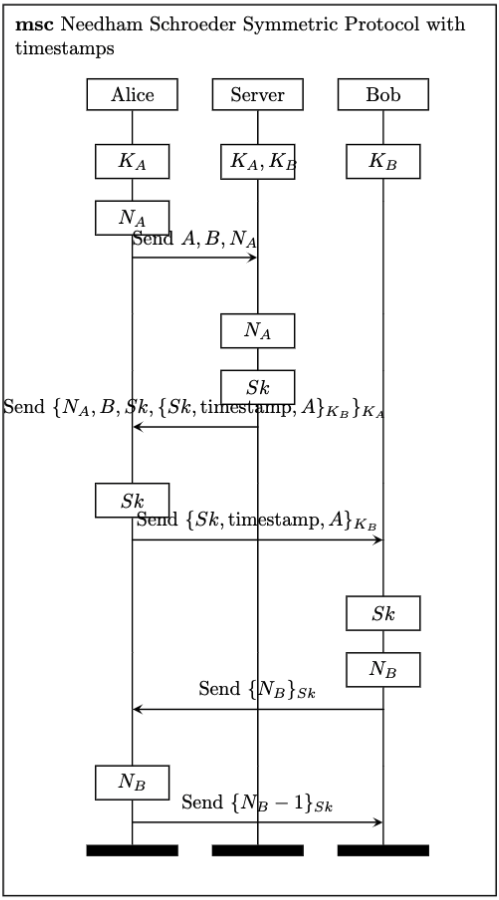
\includegraphics[width=0.45\textwidth]{Figures/NS_fixed.png}
    \label{fig:NS_fixed}
    \caption{Needham-Schroeder protocol with added timestamps}
\end{figure}
%\begin{msc}{Needham Schroeder Symmetric Protocol with timestamps}
    \declinst{alice}{}{Alice}
    \declinst{server}{}{Server}
    \declinst{bob}{}{Bob}
    \action*{ \begin{minipage}{1cm}\centering $K_A$ \end{minipage} }{alice}
    \action*{ \begin{minipage}{1cm}\centering $K_A, K_B$ \end{minipage} }{server}
    \action*{ \begin{minipage}{1cm}\centering $K_B$ \end{minipage} }{bob}
    \nextlevel[2]
    \action*{ \begin{minipage}{1cm}\centering $N_A$ \end{minipage} }{alice}
    \nextlevel[2]
    \mess{Send $A, B, N_A$}{alice}{server}
    \nextlevel[2]
    \action*{ \begin{minipage}{1cm}\centering $N_A$ \end{minipage} }{server}
    \nextlevel[2]
    \action*{ \begin{minipage}{1cm}\centering $Sk$ \end{minipage} }{server}
    \nextlevel[2]
    \mess{Send $\{N_A, B, Sk, \{Sk, \textrm{timestamp}, A\}_{K_B} \}_{K_A}$}{server}{alice}
    \nextlevel[2]
    \action*{ \begin{minipage}{1cm}\centering $Sk$ \end{minipage} }{alice}
    \nextlevel[2]
    \mess{Send $\{Sk, \textrm{timestamp}, A\}_{K_B}$}{alice}{bob}
    \nextlevel[2]
    \action*{ \begin{minipage}{1cm}\centering $Sk$ \end{minipage} }{bob}
    \nextlevel[2]
    \action*{ \begin{minipage}{1cm}\centering $N_B$ \end{minipage} }{bob}
    \nextlevel[2]
    \mess{Send $\{N_B\}_{Sk}$}{bob}{alice}
    \nextlevel[2]
    \action*{ \begin{minipage}{1cm}\centering $N_B$ \end{minipage} }{alice}
    \nextlevel[2]
    \mess{Send $\{N_B-1\}_{Sk}$}{alice}{bob}
\end{msc}

To model this version of the protocol we must change the rules that formalize the intermediate exchanges to include such timestamps:

\begin{lstlisting}[language=Tamarin]
rule Server_answers_request :
    let
        message_to_bob = senc(<~sk, ~timestamp, alice>, kb)
        message_to_alice = senc(<nonce, bob, ~sk, message_to_bob>, ka)
    in
    [
        !Server(alice, ka),
        !Client(alice, ka),
        !Client(bob, kb),
        In(<alice, bob, nonce>),
        Fr(~sk),
        Fr(~timestamp)
    ]
    --[ ServerSendsToAlice(message_to_alice),
        Secret(~sk) ]->
    [
        Out(message_to_alice)
    ]
\end{lstlisting}

\begin{lstlisting}[language=Tamarin]
rule Alice_receives_answer :
    let
        message_to_bob = senc(<sk1, timestamp, alice>, k)
        message_to_alice = senc(<nonce, bob, sk, message_to_bob>, ka)
    in
    [
        !Client(alice, ka),
        !Client(bob, kb),
        AliceQueriesServer(alice, bob, nonce),
        In(message_to_alice)
    ]
    --[ AliceReceivesAnswer(message_to_alice, nonce, message_to_bob, sk, ka),
        AliceSendsToBob(message_to_bob),
        SecretEstablished(alice, bob, sk) ]->
    [
        ExchangeInitiated(alice, bob, sk),
        Out(message_to_bob)
    ]
\end{lstlisting}

\begin{lstlisting}[language=Tamarin]
rule Bob_responds_to_Alice :
    let
        message_from_alice = senc(<sk, timestamp, alice>, kb)
        encrypted_nonce = senc(~nonce, sk)
    in
    [
        In(message_from_alice),
        Fr(~nonce),
        !Client(alice, ka),
        !Client(bob, kb),
        !Server(bob, kb)
    ]
    --[ BobReceivesFromAlice(message_from_alice, sk, kb),
        SecretEstablished(bob, alice, sk, timestamp),
        BobSendsNonce(encrypted_nonce) ]->
    [
        SessionPending(bob, alice, ~nonce, sk),
        Out(encrypted_nonce)
    ]
\end{lstlisting}

We also must introduce a new restriction that models the checking of the timestamp by Bob:

\begin{lstlisting}[language=Tamarin]
restriction CheckingTimestamps :
    "All alice bob sk timestamp #t1 #t2 .
        SecretEstablishedWithTimestamp(bob, alice, sk, timestamp) @ #t1 &
        SecretEstablishedWithTimestamp(bob, alice, sk, timestamp) @ #t2
            ==> #t1 = #t2"
\end{lstlisting}

We can see now that Tamarin when run on the \lstinline|Attack| lemma is not able now to provide any valid trace, thus confirming that this attacks was solved.

\subsubsection{Perfomance metrics}

By running Tamarin on the files that contain the theories formalizing the protocol in the two forms, we will obtain the evaluation of the formulas modeling the security properties. Assuming that we want to analyze the theory of the unfixed Needham-Schroeder protocol contained in \lstinline|./NS.spthy|, we will obtain the following output:

\begin{lstlisting}[language=Terminal]
>>> tamarin-prover NS.spthy

================================================
summary of summaries:

analyzed: NS.spthy

  types (all-traces): verified (45 steps)
  Sanity (exists-trace): verified (15 steps)
  Confidentiality (all-traces): verified (64 steps)
  Attack (exists-trace): verified (18 steps)

================================================
\end{lstlisting}

Similarly, by analyzing the formalization of the fixed protocol contained within file \lstinline|./NS_fixed.spthy|, the tool provides the following result:

\begin{lstlisting}[language=Terminal]
>>> tamarin-prover NS_fixed.spthy

================================================
summary of summaries:

analyzed: NS_fixed.spthy

  types (all-traces): verified (130 steps)
  Sanity (exists-trace): verified (15 steps)
  Confidentiality (all-traces): verified (19 steps)
  Attack (exists-trace): falsified - no trace found (294 steps)

================================================
\end{lstlisting}

In order to gain some insight on the tool's performance, we can measure the time and space resources required by a series of executions of the prover on the single lemmas and calculate some statistics on it. Automating such procedure is pretty straightforward in any modern programming language, and in our case we chose to use Python along to GNU's \lstinline|time| command line utility \cite{GNUtime}:

\begin{lstlisting}
import subprocess, re, json
from statistics import mean, stdev

def runTamarin(filename, lemmaName) :
    command = f'gtime tamarin-prover {filename}.spthy --prove={lemmaName}'
    process = subprocess.run(command.split(), stdout=subprocess.PIPE, stderr=subprocess.PIPE, universal_newlines=True)
    gtimeResults = process.stderr.split('\n')[-3].split()
    time = list(map(int, re.split('\:|\.', gtimeResults[2][:-7])))
    milliseconds = (time[0] * 60 * 1000) + (time[1] * 1000) + (time[2] * 10)
    maxMemory = int(gtimeResults[-1][:-13])
    return milliseconds, maxMemory

FILES = ['NS', 'NS_fixed']
LEMMAS = ['types', 'Sanity', 'Confidentiality', 'Attack']
N_ITERATIONS = 100

results = {}

for file in FILES :
    for lemma in LEMMAS :
        times = []
        memories = []
        for i in range(N_ITERATIONS) :
            print(f'Lemma: {lemma} | Iteration: {i+1}/{N_ITERATIONS}')
            newTime, newMemory = runTamarin(file, LEMMAS[0])
            times.append(newTime)
            memories.append(newMemory)
        results[lemma] = {}
        results[lemma]['maxTime'] = max(times)
        results[lemma]['maxMemory'] = max(memories)
        results[lemma]['minTime'] = min(times)
        results[lemma]['minMemory'] = min(memories)
        results[lemma]['avgTime'] = mean(times)
        results[lemma]['avgMemory'] = mean(memories)
        results[lemma]['stdevTime'] = stdev(times)
        results[lemma]['stdevMemory'] = stdev(memories)
    with open(f'benchmarks_{file}.json', 'w') as f:
        json.dump(results, f)
\end{lstlisting}

The script described above measures the resources used to prove each lemma during 100 different iterations. Note that each iteration requires a precomputation-phase overhead, which could be easily amortized by computing all the lemmas in the same execution. The results of our experimentation as described in tables \ref{tab:tableNS} and \ref{tab:tableNSFixed}.

\begin{table*}
    \centering
    \resizebox{0.8\textwidth}{!}{
    {\renewcommand{\arraystretch}{1.5}%
    \begin{tabular}{@{}lcccccccccc@{}}
        \toprule
        \multicolumn{1}{c}{} & \multicolumn{1}{c}{} & \multicolumn{4}{c}{Duration [ms]} & \multicolumn{4}{c}{Peak RAM usage [kB]}\\
        \cmidrule(rl){4-7} \cmidrule(rl){8-11}
        Lemma & \# of steps & Mean & Max & Min & Deviation & Mean & Max & Min & Deviation \\
        \midrule
        types & 123 & 697 & 770 & 660 & 15.09 & 46697 & 51248 & 44976 & 1295.62\\
        Sanity & 15 & 701 & 800 & 670 & 18.20 & 46973 & 50208 & 44016 & 1316.64\\
        Confidentiality & 98 & 706 & 770 & 660 & 14.75 & 46957 & 50224 & 43984 & 1357.73\\
        Attack & 19 & 745 & 800 & 710 & 16.60 & 46702 & 51232 & 44992 & 1340.96\\
        \bottomrule
        \end{tabular}
    }}
    \caption{Tamarin's performances during the verification of the Needham Schoroeder Symmetric protocol}
    \label{tab:tableNS}
\end{table*}

\begin{table*}
    \centering
    \resizebox{0.8\textwidth}{!}{
    {\renewcommand{\arraystretch}{1.5}%
    \begin{tabular}{@{}lcccccccccc@{}}
        \toprule
        \multicolumn{1}{c}{} & \multicolumn{1}{c}{} & \multicolumn{4}{c}{Duration [ms]} & \multicolumn{4}{c}{Peak RAM usage [kB]}\\
        \cmidrule(rl){4-7} \cmidrule(rl){8-11}
        Lemma & \# of steps & Mean & Max & Min & Deviation & Mean & Max & Min & Deviation \\
        \midrule
        types & 130 & 912 & 1000 & 850 & 37.11 & 61134 & 63504 & 58352 & 875.15\\
        Sanity & 15 & 935 & 990 & 870 & 24.51 & 61155 & 62528 & 58288 & 912.24\\
        Confidentiality & 19 & 953 & 1040 & 900 & 28.58 & 61132 & 62496 & 59360 & 761.72\\
        Attack & 294 & 989 & 1510 & 890 & 86.09 & 61195 & 64528 & 59376 & 786.25\\
        \bottomrule
        \end{tabular}
    }}
    \caption{Tamarin's performances during the verification of the Needham Schoroeder Symmetric protocol after fixing}
    \label{tab:tableNSFixed}
\end{table*}

As we can see, with this toy-protocol example, Tamarin is able to prove all the properties in the blink of an eye. Of course, when considering more complex formalizations with additional rules and bigger equational theories involved (such as the \lstinline|diffie-hellman| or the \lstinline|xor| built-ins), the proving process becomes more time-consuming (and often non-terminating). For example, in the reference GitHub repository \cite{github} for this paper it is also possible to find a Tamarin formalization of the X3DH exchange proposed by Marlinspike and Perrin \cite{x3dh} that, despite its brevity, manages to get the prover stuck during the precomputation phase due to the high number of Diffie Hellman exchanges required in the protocol.

\section{Conclusions}\label{sec:conclusions}

In this essay we managed to present the Tamarin prover with a top-down approach: starting from a general introduction to the formal checking context background (in particular the symbolic model for protocol verification), we introduced the famous theorem prover by quickly explaining its syntax and usage. In order to provide a more concrete point of view on the matter, we also presented the Needham Schroeder Symmetric protocol and formalized its message exchange in Tamarin semantics. Then, we used the tool to prove some of its security properties and showed how it could be subject to a simple replay attack. After showing a potential fix to the problem, we proved that the proposed modification did, in fact, eliminated the attack. Finally, we provided some performance metrics on the tool.

The topic of automated formal verification of protocols is currently an area of active research within the symbolic artificial intelligence field. As computer scientists, this allows us to go through a less cumbersome verification process when checking protocols for correctness, while as users this provides us a better sense of trust with regards to the security features of the application we are using, since their exchanges are more easily formalized and verified against attackers.

%----------------------------------------------------------------------------------------
%	ACKNOWLEDGEMENTS
%----------------------------------------------------------------------------------------

% \phantomsection
% \section*{Acknowledgments} % The \section*{} command stops section numbering
% 
% \addcontentsline{toc}{section}{Acknowledgments} % Adds this section to the table of contents
% 
% So long and thanks for all the fish \cite{Figueredo:2009dg, Smith:2012qr}.

%----------------------------------------------------------------------------------------
%	REFERENCE LIST
%----------------------------------------------------------------------------------------

\phantomsection
\bibliographystyle{alpha}
\bibliography{references.bib}

%----------------------------------------------------------------------------------------

\end{document}